\documentclass[12pt]{article}
\usepackage{cite}
\usepackage{graphicx}
\usepackage{geometry}
\usepackage{float}
\usepackage{multicol}
\usepackage{subfigure}

\geometry{left=2.0cm,right=2.0cm,top=2.5cm,bottom=2.5cm}

\title{
    \textbf{\Huge ECE385} \\
    \huge Fall 2020 \\
    \huge Final Report \\[120pt]
    \textbf{\Huge Game: I Wanna an A in ECE385} \\[120pt]
    }

\author{
    \large Name: Zhou Qinren \\ 
            \quad\qquad Zhang Yichi \\ 
    \large Lab Section: LA3 \\ 
    \large TA's Name: Yu Yuqi
    }

\date{Jan. $2^{nd}$ 2021}

\begin{document}
\setlength{\parindent}{0pt}
\maketitle
\newpage

\section{Written Description}
\subsection{The Purpose of the Circuit}
Our project is a game named ‘I wanna’. The player controls the motion of the game character and has to escape traps and reach the final point. 

There are mainly three parts of the circuits, the game logic, game display and keyboard interaction. We used the hardware to implement logic control, such as barrier test and death test. We also used color mapper and vga controller to display on the screen. The color mapper is capable of painting graphs that are stored in on-chip memory. Software (Nios) is used to fulfill keyboard interaction. We modified the C code in lab8 so as to receive multiple keyboard presses at the same time. 

\subsection{Features}
We fulfilled all the features we listed in the proposal. \\

1.	The game character is well displayed on the screen. He has 4 states in total, still, moving, jumping, and falling. Each state is demonstrated by a different set of graphs. For example, the moving state has 4 graphs, and when the character is moving in the x-direction, the 4 graphs are displayed periodically and fluently so that the player sees a series of motion pictures. \\

2.	The game has appropriate death check and collision check, which guarantee the game experience. If the game character falls into a trap, the logic circuit determines his death, and a ‘game over’ scene will be displayed, until the player press ‘R’ keycode to restart the game from the latest checkpoint. The collision check assures that the character cannot run into the barriers, such as a box, or the ground under his feet. \\

3.	The player controls the motion of the game character through keyboard. ‘W’ is for jumping, ‘A’ for moving left, ‘D’ for moving right, ‘R’ for restart from the latest checkpoint, ‘J’ for shooting. There is a hidden instruction that when the player types ‘final a’ in a sequence, the game character will go into god-mode, where he cannot be killed. \\

4.	The game maintains a death counter to count the number of times the character dies (fallen into a trap). The counter is set to 0 on each time the whole hardware is reset through KEY0 on the DE2 board. Each time the player presses ‘R’ keycode to restart from the latest checkpoint, the death counter increment itself. \\

5.	The player can shoot at some barriers so as to destroy them. Moreover, in the last scene, the player has to shoot at a red target, otherwise he can never reach the final point. \\

6.	The game has some sound effects. There are 3 sounds in total, shooting sound, game over, and victory, and all of which are triggered by player behavior. The sound effect module is actually written by others, which we found on the github. Our contribution is to write a sound control program, so that the sound module plays the music we desire. \\

7.	The game has some checkpoints. The player can return to the latest checkpoint by pressing ‘R’ keycode. We add this function to decrease game difficulty. \\

8.	Some traps in the game might surprise, or even annoy the player quite a lot. These traps serve as pranks. \\

9.	There are two levels of difficulty. If the player feels that the game is too hard, then he can type the hidden code ‘finala’, and then the character goes into god-mode. \\


\subsection{Inputs/Outputs}
Two fundamental inputs from the DE2 board:
Input logic CLOCK\_50,
Input logic [3:0] KEY; \\

VGA interface:
Output logic [7:0] VGA\_R, VGA\_G, VGA\_B, 
Output logic VGA\_CLK, VGA\_SYNC\_N, VGA\_BLANK\_N, VGA\_VS, VGA\_HS; \\

CY7C67200 interface:
Inout wire [15:0] OTG\_DATA
Output logic [1:0] OTG\_ADDR,
Output logic OTG\_CS\_N, OTG\_RD\_N, OTG\_WR\_N, OTG\_RST\_N
Input logic OTG\_INT; \\

SDRAM interface for Nios II software:
Output logic [12:0] DRAM\_ADDR,
Inout wire [31:0] DRAM\_DQ, 
Output logic [1:0] DRAM\_BA,
Output logic [3:0] DRAM\_DQM,
Output logic DRAM\_RAS\_N, DRAM\_CAS\_N, DRAM\_CKE, DRAM\_WE\_N, DRAM\_CS\_N, DRAM\_CLK; \\

WM8731 audio interface:
Inout wire I2C\_SDAT,
Output logic I2C\_SCLK, AUD\_XCK, AUD\_BCLK, AUD\_DACLRCK, AUD\_DACDAA; \\

\subsection{Process of the Inputs/Outputs}
CLOCK\_50 serves as the clock of the flip-flop content. KEY0 is the reset button that resets the whole hardware.

CY7C67200 interface is the interaction module between the Nios and FPGA. The Nios reads keycode and send the signals to the FPGA. It is the same as in lab 8 except our design can receive multiple keycodes at the same time. These inputs and outputs listed above are control signals to transfer data between Nios and FPGA.

SDRAM interface is the same as in previous lab.

VGA interface are some signals necessary to display on the screen. Our game logic will produce the correct RGB signals for each pixel. It is similar to lab 8, except our design is much more complicated, and we use on-chip memory to store the graphs.

WM8731 audio interface configurate the audio device first. Then our game logic will send correct output to the device, so as to play the sound. 

\subsection{Outputs Shown}
The screen should correctly display the game character, traps and background. The character should move in the direction or jump as the player instructs. If the character falls into a trap, a game over graph should be displayed, until the player press ‘R’ keycode to restart. The character should not be able to cross a barrier. The audio should play some sounds when the character shoots, fails or succeeds. In general, all the features listed above should be correctly displayed. 

\section{Module Description}
\textbf{Module}: man \\ 
\textbf{Inputs}: Clk, Reset, frame\_clk, [1:0] move, [3:0] barrier, jump, dead, check, restart, [9:0] mapX, [9:0] mapY, reset1, reset2, reset3 \\ 
\textbf{Outputs}: [9:0] man\_x, [9:0] man\_y, [1:0] man\_state, [1:0] man\_graph\_counter, is\_right, is\_dead, checking \\
\textbf{Description}: This module is the control unit of the man behavior. Everything important is stored in some registers, and Clk is used to maintain the flip-flop behavior. frame\_clk is the 60 Hz signal, which is used to indicate the flip-flops should change values. The inputs are generally some control signals. 

Move is a 2-bit signal, indicating x-motion. 00 stands for staying still, 01 for moving to the right, and 10 for moving to the left.

Barrier is a 4-bit signal, indicating whether a barrier surrounds the man. The 4 bits are interpreted as low, up, left, right, and 1 means a barrier exists. For example, if there is a barrier on the right side, then the rightmost bit is 1. 0 means the man can freely move in the corresponding direction. 

Jump is high when the player input a jump instruction, which is the ‘w’ keycode, and low otherwise. 

Dead is high when other modules determines the man has been killed by some traps. 

Check is high when the man has reached some checkpoints, and the man module will update the coordinates of the checkpoints.
Restart is high when the player input a restart instruction, which is the ‘r’ keycode, and the man will return to the latest checkpoint. 

mapX, mapY are the coordinates of the checkpoints. 

Reset1, reset2, and reset3 are some trigger signals which indicate the man has entered a new scene, and the man module will reset the man’s initial location.

Man\_x, man\_y are the coordinates of the man, which are used in painting the man. Man\_state indicates the current state of the man. There are four states in total, still, moving, jumping, and falling, each corresponds to a different set of graphs. Man\_graph\_counter is used to count the current graph to show on the screen. Is\_right indicates whether the man is moving right or left. Is\_dead indicates whether the man has been killed. \\ 
\textbf{Purpose}: This module is the control unit of the man behavior. the inputs are some signals to control the man, and the outputs are some signals which are necessary for painting the man in the right location and status. \\

\textbf{Module}: keycodeDecoder \\ 
\textbf{Inputs}: Clk, Reset, [31:0] keycode \\ 
\textbf{Outputs}: [1:0] move, jump, restart, shoot, god \\
\textbf{Description}: Some important information is stored in registers, and Clk is used to refresh the contents. We modified the C code in Nios, and thus our program can take four keycodes at the same time. We also modified the PIO in platform so that it can transfer information in 32 bits ( 8bit / each *  4). [31:0] Keycode is the signals obtained by PIO, and then we decode it to recognize the instructions input by the player. 

[1:0] move is used to instruct the man’s x-motion. The keycode ‘d’ indicates moving right, and ‘a’ indicates moving left. Jump is the ‘w’ keycode. Restart is the ‘r’ keycode, and shoot is the ‘j’ keycode. God is a hidden instruction, which is active when the player inputs ‘final A’ in a sequence. When god is active, the man is in the god mode ---- he cannot be killed. \\ 
\textbf{Purpose}: This module is used to decode the user input keycodes and send control signals to other modules. \\

\textbf{Module}: death\_counter \\ 
\textbf{Inputs}: Clk, frame\_clk, Reset, is\_dead \\ 
\textbf{Outputs}: tenths, ones \\
\textbf{Description}: Some important information is stored in registers, and Clk is used to refresh the contents. frame\_clk is the 60 Hz signal, which is used to indicate the flip-flops should change values.

Is\_dead is the signal sending from man.sv, indicating the man has been killed. The death\_coutner.sv module counts the number of deaths, and store it in tenths and ones.

For example, the current number of deaths is 37, then tenths outputs 3, and ones outputs 7. \\ 
\textbf{Purpose}: This module counts the number of deaths, and outputs this number so that the color mapper could paint this number. \\

\textbf{Module}: bullets \\ 
\textbf{Inputs}: bullets.sv
Inputs: Clk, frame\_clk, shoot, [9:0] man\_x, [9:0] man\_y, is\_right, bullet1\_off, bullet2\_off, bullet3\_off \\ 
\textbf{Outputs}: bullet, [9:0] bullet1\_x, [9:0] bullet1\_y, [9:0] bullet2\_x, [9:0] bullet2\_y, [9:0] bullet3\_x, [9:0] bullet3\_y, bullet1\_active, bullet2\_active, bullet3\_active \\
\textbf{Description}: Some important information is stored in registers, and Clk is used to refresh the contents. frame\_clk is the 60 Hz signal, which is used to indicate the flip-flops should change values.

Shoot is the ‘j’ keycode, indicating the shooting instruction input by the player. 
Man\_x and man\_y are the man’s current location. The bullets should be at the same location as the man if they have not been shot.

Is\_right indicates the direction of x-motion.

Bullet1\_off indicates the bullet has intersected with a barrier, and the bullet should not be shown. It is identical for bullet2\_off and bullet3\_off.
Bullet is the signal connecting with the sound control, so that the audio device can play the shooting sound.

Bullet1\_x and bullet1\_y are the location of the bullet1. Bullet1\_active tells the color mapper whether the bullet should be shown or not. \\ 
\textbf{Purpose}: This module controls the bullet behaviors. We maintain three bullets, and their location and active status are sending to the color mapper, which will decide whether the bullets should be shown or where to show. \\

\textbf{Module}: sound\_control \\ 
\textbf{Inputs}: Clk, Reset, bullet, gameover, victory \\ 
\textbf{Outputs}: [2:0] sound\_select \\
\textbf{Description}: bullet, gameover, and victory indicates which sound should be played. We used some modules found on github that are written by others, and some mif files. These files include Sound\_Top, SoundROM\_win.v, SoundROM\_gameover.v, SoundROM\_coin.v, and the corresponding mif files. The sound\_control.sv is written by ourselves, which handles Sound\_Top so that the audio device plays the sounds we desire. The Sound\_Top module is well written by others, and we only have to input the sound\_select signal. \\ 
\textbf{Purpose}: Make some sound effect when the player shoots, fails or succeeds. \\

\textbf{Module}: randomCounter \\ 
\textbf{Inputs}: Clk, frame\_clk, Reset, hit, restart \\ 
\textbf{Outputs}: thorn1, thorn2, thorn3, thorn4 \\
\textbf{Description}: Hit is high when the bullet hits the target. 

Restart is high when the man has returned to the checkpoint. 

Thorn1 is high when the trap should be displayed, and 0 if it should not.
The same for thorn2, thorn3, and thorn4. \\ 
\textbf{Purpose}: This module serves as a random mechanism. There are four traps in total, and when the player hits the target, some traps will vanished randomly. \\

\textbf{Module}: kid\_idle \\ 
\textbf{Inputs}: [11:0] read\_address, Clk \\ 
\textbf{Outputs}: [3:0] data\_Out \\
\textbf{Description}: It periodically outputs a 4-bit color stored in the on-chip memory based on the 12-bit input address. There are 104x23=2392 pixels, thus, we need 12 bits. \\ 
\textbf{Purpose}: This module controls an on-chip memory that stores four images of the game character kid when he is idle. Therefore, when kid is idle, four images of kid will be shown on the screen periodically like he is wobbling. \\

\textbf{Module}: kid\_walk \\ 
\textbf{Inputs}: [11:0] read\_address, Clk \\ 
\textbf{Outputs}: [3:0] data\_Out \\
\textbf{Description}: It periodically outputs a 4-bit color stored in the on-chip memory based on the 12-bit input address. There are 104x23=2392 pixels, thus, we need 12 bits. \\ 
\textbf{Purpose}: This module controls an on-chip memory that stores four images of the game character kid when he is walking. Therefore, when kid is idle, four images of kid will be shown on the screen periodically like he is walking. \\

\textbf{Module}: kid\_jump \\
\textbf{Inputs}: [10:0] read\_address, Clk \\ 
\textbf{Outputs}: [3:0] data\_Out \\
\textbf{Description}: It periodically outputs a 4-bit color stored in the on-chip memory based on the 11-bit input address. There are 52x25=1300 pixels, thus, we need 11 bits. \\ 
\textbf{Purpose}: This module controls an on-chip memory that stores one image of the game character kid when he is jumping and one when he is falling. Therefore, when kid is jumping and falling, the specific images of kid will be shown on the screen. \\

\textbf{Module}: background \\
\textbf{Inputs}: [18:0] read\_address, Clk \\ 
\textbf{Outputs}: [3:0] data\_Out \\
\textbf{Description}: It periodically outputs a 4-bit color stored in the on-chip memory based on the 19-bit input address. There are 640x480=307200 pixels, thus, we need 19 bits. \\ 
\textbf{Purpose}: This module controls an on-chip memory that stores the bonus scene, a pixelated image of our mentor of ECE385, Li Chushan, that will be shown when the player pass the whole game. \\

\textbf{Module}: spike \\
\textbf{Inputs}: [11:0] read\_address, Clk \\ 
\textbf{Outputs}: [3:0] data\_Out \\
\textbf{Description}: It periodically outputs a 4-bit color stored in the on-chip memory based on the 12-bit input address. There are 128x32=4096 pixels, thus, we need 12 bits. \\ 
\textbf{Purpose}: This module controls an on-chip memory that stores four images of the spike towards different directions. There will be another variable, spikestate, to determine which direction will be used and shown on the screen. \\

\textbf{Module}: block \\
\textbf{Inputs}: [9:0] read\_address, Clk \\ 
\textbf{Outputs}: [3:0] data\_Out \\
\textbf{Description}: It periodically outputs a 4-bit color stored in the on-chip memory based on the 10-bit input address. There are 32x32=1024 pixels, thus, we need 10 bits. \\ 
\textbf{Purpose}: This module controls an on-chip memory that stores the image of the block. The blocks will block the kid from moving. \\

\textbf{Module}: checkpoint \\
\textbf{Inputs}: [10:0] read\_address, Clk \\ 
\textbf{Outputs}: [3:0] data\_Out \\
\textbf{Description}: It periodically outputs a 4-bit color stored in the on-chip memory based on the 11-bit input address. There are 64x32=2048 pixels, thus, we need 11 bits. \\ 
\textbf{Purpose}: This module controls an on-chip memory that stores two images of the checkpoint. One with a red light in the middle, another with a green one. When the kid is touching the checkpoint, we will output the 4-bit color of the green one. Otherwise, we will output the 4-bit color of the red one. \\

\textbf{Module}: dead \\
\textbf{Inputs}: [14:0] read\_address, Clk \\ 
\textbf{Outputs}: [3:0] data\_Out \\
\textbf{Description}: It periodically outputs a 4-bit color stored in the on-chip memory based on the 15-bit input address. There are 320x66=21120 pixels, thus, we need 15 bits. \\ 
\textbf{Purpose}: This module controls an on-chip memory that stores the scene that will appear on the screen when the character kid is dead. \\

\textbf{Module}: paint\_background \\ 
\textbf{Inputs}: [3:0] bgcolor \\ 
\textbf{Outputs}: [7:0] r,g,b \\
\textbf{Description}: It converts a 4-bit color code to three real 8-bit RGB color signals. \\ 
\textbf{Purpose}: This module helps to get real RGB values for the background image of the bonus scene. \\

\textbf{Module}: map \\ 
\textbf{Inputs}: Clk, Reset, restart, thorn1, thorn2, thorn3, thorn4, [9:0] DrawX, [9:0] DrawY, [9:0] man\_x, [9:0] man\_y \\ 
\textbf{Outputs}: is\_block, is\_spike, is\_check, reset1, reset2, reset3, victory, button, [9:0] mapx, [9:0] mapy, [1:0] mapspikestate, [1:0] inmap, [3:0] barrier \\
\textbf{Description}: It converts a 640x480 pixels screen to a 20x15 blocks map with each block 32x32 pixels because the sprites of the blocks, spikes, checkpoints are all 32x32 pixels. Then it outputs mapx and mapy which is the upper left corner of the current block according to the DrawX and DrawY. We create a 20x15x2x2 bits variable map inside to store the state of each block since we have 2 20x15-block maps and 00 stands for nothing on the map, 01 stands for blocks, 10 stands for spikes, 11 stands for checkpoints. For spikes, we create another spikemap with the same size to store the direction of the spikes and 00 means up, 01 means right, 10 means left, 11 means down. According to the mapx and mapy, we check the corresponding values in the map and spikemap to determine whether the current block is a block, a spike or a checkpoint and if it is a spike what is the direction of the spike and finally output the results as signals is\_block, is\_spike, is\_check and mapspikestate. Since we have 2 maps and a bonus scene, we outputs a variable inmap to show the map the character is currently in (00 for map0, 01 for map1, 10 for bonus scene of victory), 3 reset signals and a variable victory to tell that the character is going from one map to another. In addition, it calls the module barrier\_detect to determine the barrier signals for the kid. Also, 4 blocks are marked as thorns and one block is marked as button for a specific trap. \\ 
\textbf{Purpose}: The purpose of this module is to create maps and some traps inside and tell the outside what the current block is, which map the character is currently in, what the current barriers are for kid's movement, whether the kid is going to another map. \\

\textbf{Module}: barrier\_detect \\ 
\textbf{Inputs}: [1:0] inmap, [1:0] map [599:0], [9:0] man\_x, [9:0] man\_y \\ 
\textbf{Outputs}: [3:0] barrier \\
\textbf{Description}: According to the image of the character kid, we pick three pixels for each direction for barrier detection. When one of the three pixels touch the block, we turn on the barrier signal and stop the kid from keeping moving in this direction. For the bonus scene of victory, we set the barriers to be the boundary of the screen. \\ 
\textbf{Purpose}: This module is a barrier detection that prevents the kid from walking into the blocks and out of the screen. \\

\textbf{Module}: flytrap \\ 
\textbf{Inputs}: Clk, Reset, restart, frame\_clk, [9:0] init\_x, [9:0] init\_y, [9:0] trigger\_x\_left, [9:0] trigger\_x\_right, [9:0] trigger\_y\_up, [9:0] trigger\_y\_down, [9:0] man\_x, [9:0] man\_y, [1:0] direction, [1:0] inmap, [3:0] speed \\ 
\textbf{Outputs}: trap\_on, [1:0] trapspikestate, [9:0] trap\_x, [9:0] trap\_y \\
\textbf{Description}: We create a spike at init\_x and init\_y. When the man\_x is between trigger\_x\_left and trigger\_x\_right and man\_y is between trigger\_y\_up and trigger\_y\_down, we turn on the output signal trap\_on and make the spike fly with a velocity equal to the speed signal and the direction based on the direction signal (00 for up, 01 for right, 10 for left, 11 for down). There will be a 6-bit counter inside to control the distance the spike flies. When the counter counts to 6'b1111111, the spike will disappear. Therefore, we output signal trap\_on to tell whether the trap is triggered, trapspikestate to tell which direction the spike points at and trap\_x and trap\_y to tell the position of the trap. Inputs Reset and restart will reset the trap. \\ 
\textbf{Purpose}: This module is to initialize and control a fly spike. Fly spikes will appear on the screen and fly towards certain direction for certain distance when the kid walks to some place and triggers it. \\

\textbf{Module}: weaktrap \\ 
\textbf{Inputs}: getshot, Clk, Reset,restart, [1:0] direction, [1:0] inmap, [9:0] init\_x, [9:0] init\_y \\ 
\textbf{Outputs}: trap\_on, [1:0] trapspikestate, [9:0] trap\_x, [9:0] trap\_y \\
\textbf{Description}: We create a weak spike at init\_x and init\_y. When the character kid shoot the spike, the input getshot will be high and the 2-bit counter inside the module will count the times it get shot. When the counter counts to 2'b11, the trap will disappear. Therefore, we output signal trap\_on to tell whether the trap is triggered, trapspikestate to tell which direction the spike points at and trap\_x and trap\_y to tell the position of the trap. Inputs Reset and restart will reset the trap. \\ 
\textbf{Purpose}: This module is to initialize and control a weak spike that can be shot by the character kid and will be disappear after some shots. \\

\textbf{Module}: istrap \\ 
\textbf{Inputs}: Reset, frame\_clk, restart, Clk, getshot2, getshot3, getshot4, getshot5, getshot6, getshot7, [1:0] inmap, [9:0] DrawX, [9:0] DrawY, [9:0] man\_x, [9:0] man\_y \\ 
\textbf{Outputs}: is\_trap, weak\_2, weak\_3, weak\_4, weak\_5, weak\_6, weak\_7, [1:0] trapspikestate, [9:0] trap\_x, [9:0] trap\_y \\
\textbf{Description}: It calls flytrap and weaktrap to initialize and control the total 11 fly and weak traps. Since there cannot be two traps overlapping at one same pixel, we determine whether the current DrawX and DrawY is a trap (is\_trap) and if it is, whether it is a weak trap (weak\_2 to weak\_7), what direction it points at (trapspikestate), what the address should be used to read out the color code from the memory (trap\_x, trap\_y). \\ 
\textbf{Purpose}: This module integrates and controls all the traps. \\

\textbf{Module}: color\_mapper \\ 
\textbf{Inputs}: Clk, frame\_clk, Reset, god,button, is\_block, is\_spike, is\_check, is\_right, is\_dead, checking, restart, bullet1\_active, bullet2\_active, bullet3\_active, is\_trap, weak\_2, weak\_3, weak\_4, weak\_5, weak\_6, weak\_7, [1:0] man\_state, [1:0] man\_graph\_counter, [1:0] mapspikestate, [1:0] inmap, [1:0] trapspikestate, [3:0] tenths, [3:0] ones, [9:0] man\_x, [9:0] man\_y, [9:0] mapx, [9:0] mapy, [9:0] DrawX, [9:0] DrawY, [9:0] bullet1\_x, [9:0] bullet1\_y, [9:0] bullet2\_x, [9:0] bullet2\_y, [9:0] bullet3\_x, [9:0] bullet3\_y, [9:0] trap\_x, [9:0] trap\_y \\ 
\textbf{Outputs}: dead, check, hit, bullet1\_off, bullet2\_off, bullet3\_off, getshot2, getshot3, getshot4, getshot5, getshot6, getshot7, [7:0] VGA\_R, [7:0] VGA\_G, [7:0] VGA\_B \\
\textbf{Description}: It calls kid\_idle, kid\_walk, kid\_jump, block, spike, checkpoint, dead, font\_rom to read out color code from these on-chip memories and store the results in 4-bit color variables we declare inside this module. It first determines the attribute of the current pixel (whether it is kid, background, bullet, block, spike, checkpoint or button) based on DrawX, DrawY, other input position signals (man\_x, man\_y, mapx, mapy, bullet\_x, bullet\_y, trap\_x, trap\_y) and attribute signals (is\_dead, checking, is\_block, is\_spike, is\_check, is\_trap). Then based on the attribute, we determine the RGB values for the current pixel. In addition, if the current pixel is the kid and is a spike and the kid's and spike's color are not white (white is the color we choose to represent transparency in the original image), we judge that the kid is dead and output a signal dead. Similarly, if the current pixel is the kid and is a checkpoint and the kid's and checkpoint's color are not white, we judge that the kid is checking and output a signal check. Similarly, if the current pixel is a bullet and is a spike and the spike's color are not white, we turn on the bullet off signal. Further, if the spike is a weak trap, we turn on the corresponding getshot signal. Similarly, if the current pixel is a bullet and is a button, we turn on the hit signal. \\
\textbf{Purpose}: This module is to process all the position signals and state signals, do the death detection, check detection and shoot detection, and determines and outputs RGB values to the VGA. It connects all the on-chip memories, the map module, man module, istrap module. \\

\textbf{Module}: VGA\_controller.sv \\ 
\textbf{Inputs}: Clk, Reset, VGA\_CLK \\ 
\textbf{Outputs}: VGA\_HS, VGA\_VS, VGA\_BLANK\_N, VGA\_SYNC\_N, [9:0] DrawX, [9:0] DrawY \\
\textbf{Description}: This module controls the VGA signals (horizontal and vertical). \\ 
\textbf{Purpose}: This module keeps tracks of the pixel that is currently under test, so that we can draw that pixel correctly. \\

\textbf{Module}: hpi\_io\_intf.sv \\ 
\textbf{Inputs}: Clk, Reset, [1:0] from\_sw\_address, [15:0] from\_sw\_data\_out, from\_sw\_r, from\_sw\_w, from\_sw\_cs, from\_sw\_reset \\ 
\textbf{Outputs}: [15:0] from\_sw\_data\_in, [1:0] OTG\_ADDR, OTG\_RD\_N, OTG\_WR\_N, OTG\_CS\_N, OTG\_RST\_N \\
\textbf{Inputs}: [15:0] OTG\_DATA \\
\textbf{Description}: This module sends some control signals to the OTG chip. \\ 
\textbf{Purpose}: This module is the hpi interface that communicates with OTG chip, it sends some control signals to the chip. These signals indicate whether to perform a read or write operation, and the address is specified. \\

\textbf{Module}: iwanna \\ 
\textbf{Inputs}: CLOCK\_50, KEY, OTG\_INT \\ 
\textbf{Outputs}: [6:0] HEX0, [6:0] HEX1, [7:0] VGA\_R, [7:0] VGA\_G, [7:0] VGA\_B, VGA\_CLK, VGA\_SYNC\_N, VGA\_BLANK\_N, VGA\_VS, VGA\_HS, [1:0] OTG\_ADDR, OTG\_CS\_N, OTG\_RD\_N, OTG\_WR\_N, OTG\_RST\_N, OTG\_INT, [12:0] DRAM\_ADDR, [1:0] DRAM\_BA, [3:0] DRAM\_DQM, DRAM\_RAS\_N, DRAM\_CAS\_N, DRAM\_CKE, DRAM\_WE\_N, DRAM\_CS\_N, DRAM\_CLK, [3:0] LEDG, I2C\_SCLK, AUD\_XCK, AUD\_BCLK, AUD\_DACLRCK, AUD\_DACDAT \\
\textbf{Inouts}: [15:0] OTG\_DATA, [31:0] DRAM\_DQ, I2C\_SDAT \\
\textbf{Description}: This is the top-level module. \\ 
\textbf{Purpose}: This module instantiates all the low-level modules, connects them properly and interacts with VGA interface, CY7C67200 interface, SDRAM interface for Nios II software and WM8731 audio interface. \\

\section{Design Procedure}
We used lab8 as the foundation of this project since I wanna is a game based on keyboard interactions. Also, we referred to Lai Xinyi's codes and audio files on github to complete our sound control components. We had asked and obtained her authorization and approval to use them. \\

To accomplish this project, we made modification to the C codes in lab8 for keyboard control and build all of the rest game logic in hardware using SystemVerlog. \\

At the beginning, we were thinking about making a game that could exhibit our abilities including basic circuits control, FSM, image processing, sound processing. Then the game I wanna came to our mind and we decided to do it. We first broke the whole game into several tasks consisting of display, motion control, collision detection, death detection, map making, trap making, sound control. We then assigned each task with a priority and made a timeline for the whole project. \\

When we started to do the project, we first searched for sprites of this game and found them in google easily. Then we divided the work. Zhou Qinren started to build the motion control for the character and Zhang Yichi started to learn the image compressing, processing and display. Further, Zhou Qinren build the keycodeDecoder (modification of lab8's hardware settings and C codes), everything with the character (motion control, shooting) and sound control. Zhang Yichi build everything related to images (display, collision detection, death detection, check detection, map making, trap making). We collaborated well. Each step of our tasks and functions are related to the next step. Only when we completed the motion control and display tasks can we continue to test the collision detection and death detection. Also, only when we completed the basic game logic can we start to create maps and traps. After the whole game can be played, we tried to add sound and more traps to polish it. 

\section{State Diagram}
\begin{figure}[H]
    \centering
    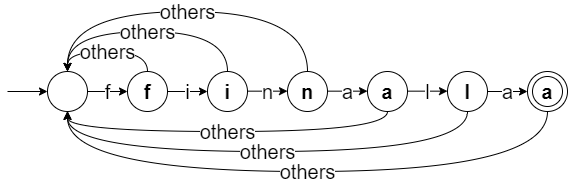
\includegraphics[width=10cm]{CheatCode.png}
    \caption{The FSM of the cheat codes.}
\end{figure}
We used an FSM to judge if the player types in the cheat code to enter the god mode.

\section{Block Diagram}
\begin{figure}[H]
    \centering
    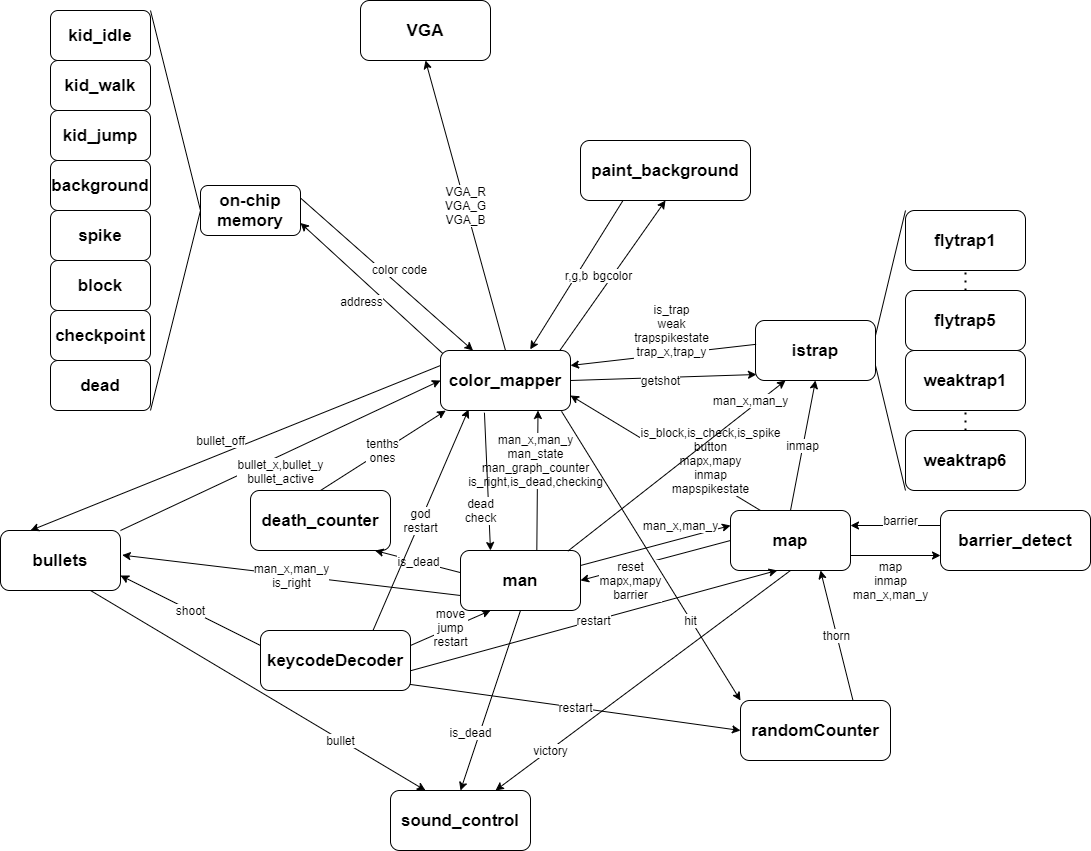
\includegraphics[width=17cm]{BlockDiagram.png}
    \caption{Block diagram in detail.}
\end{figure}
\begin{figure}[H]
    \centering
    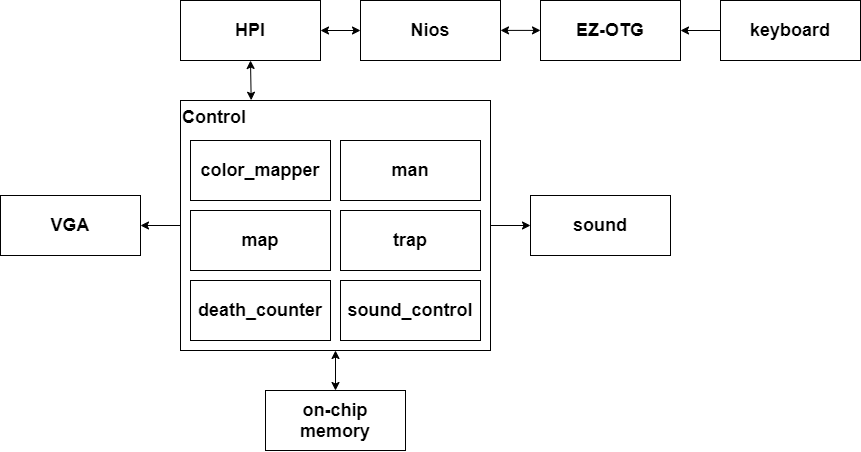
\includegraphics[width=16cm]{TopLevelView.png}
    \caption{Top level view of the project.}
\end{figure}

\section{Design Statistics}
\begin{table}[H]
    \centering
    \resizebox*{8cm}{5cm}{
        \begin{tabular}{|l|l|l|l|}
        \hline
        LUT           & 6698            \\ \hline
        DSP           & 24              \\ \hline
        BRAM          & 2678840         \\ \hline
        Flip-Flop     & 2607            \\ \hline
        Frequency     & 134.95MHz       \\ \hline
        Static Power  & 108.63mW        \\ \hline
        Dynamic Power & 0.85mW          \\ \hline
        Total Power   & 178.79mW        \\ \hline
        \end{tabular}
    }
    \caption{Design statistics table for the project.}
\end{table}

\section{Conclusion}
\subsection{Debug}
The most common bug is that the graph is displayed incorrectly. We found that the most often cause is the clock issue. Our flip-flops use the 50 MHz clock, while the screen refreshes at 60 Hz. Sometimes we misuse the two clocks, which results in some confusing bugs.
Another bug is that Quartus does not report some assignment error. For example, if we use assign statement, and assign something that is never declared to an existing signal, Quartus will not report an error. We believe this issue is a bug of Quartus itself. 

\subsection{Summary}
Every feature we listed at the beginning of this report is fulfilled. In summary, our project is a running game which interacts with the player through keyboard. The character can move according to the player’s instruction. The game has collision test and death test, it also maintains a death counter. The game also has some sound effect. 

\newpage
\bibliography{}
\bibliographystyle{ieeetr}
\end{document}